\documentclass[aspectratio=169,table,xcdraw,18pt,portugues]{beamer}

% =====================================================================
% This file's purpose is to organize dependencies, package load and
% document configuration outside the main file, which will isolate
% LaTeX code from content text. There are sections here by each
% plugin and config function. You can comment packages and configs
% if they are not necessary in your LaTeX document.
% Please, be aware that this section is invoked on the PREAMBLE,
% right after the document class.

% This document contains code only, not text content:
% spell-checker: disable

% =====================================================================
% This section defines settings related to the document pages 
% like margins and spaces.

\usepackage{fetchcls}  % Allow decisions based on class name
\usepackage{ifthen}  % Allow decisions based on conditions
\usepackage{afterpage}  % Allow other packages to apply logic by page
\usepackage{geometry}  % This package allows selecting margins size
\usepackage{setspace}  % Allows selecting line spacing
\usepackage{anyfontsize}  % Allows custom font sizes

% =====================================================================
% This section is dedicated to graphical elements, like formulas
% and images. The packages here helps to configure those visual
% elements.

% American Mathematical Society packages:
\usepackage{amsmath}
\usepackage{amsfonts}
\usepackage{amsthm}

% To have acronyms and glossaries working:
\usepackage[printonlyused]{acronym}
% \renewcommand*\acffont{\textit}  % change the style of long acms
% \renewcommand*\acsfont{\textit}  % change the style of short acms

% Use and create colors definitions (with tables support moved to beamer):
\usepackage{xcolor}

% Insert pictures, make drawings and plots:
\usepackage{graphicx}
\usepackage{tikz}
\usepackage{pgfplots}
\pgfplotsset{compat=1.16}

% Save your images here:
\graphicspath{ {./images/} }

% This will define colors that can be used as a theme:
\definecolor{fgcolor}{HTML}{005B90}
\definecolor{bgcolor}{HTML}{FFFFFF}
\definecolor{c1color}{HTML}{00BAEA}
\definecolor{c2color}{HTML}{6E6E70}
\definecolor{c3color}{HTML}{F0F0F6}

% This will set the theme aspect by changing sizes and colors:
\setbeamerfont{title}{size=\Huge}  % Title slides
\setbeamerfont{subtitle}{size=\Large}
\setbeamerfont{author}{size=\normalsize}
\setbeamerfont{institute}{size=\large}
\setbeamerfont{date}{size=\tiny}
\setbeamerfont{footline}{size=\tiny}
%
\setbeamerfont{frametitle}{size=\Large}  % Regular slides
\setbeamerfont{framesubtitle}{size=\small}
%
\setbeamercolor*{background canvas}{bg=bgcolor}  % Colors
\setbeamercolor*{title}{fg=c1color}
\setbeamercolor*{subtitle}{fg=c1color}
\setbeamercolor*{author}{fg=c1color}

\setbeamercolor*{footline}{fg=c2color}
\setbeamercolor{frametitle-left}{fg=c1color}
\setbeamercolor{frametitle}{fg=c1color}
\setbeamercolor*{itemize item}{fg=c1color}
\setbeamercolor*{itemize subitem}{fg=c1color}
\setbeamercolor*{normal text}{fg=fgcolor}
\setbeamercolor{bibliography item}{fg=c1color}
\setbeamercolor{bibliography entry author}{fg=fgcolor}
\setbeamercolor{bibliography entry title}{fg=fgcolor}
\setbeamercolor{bibliography entry location}{fg=fgcolor}
\setbeamercolor{bibliography entry note}{fg=fgcolor}

% =====================================================================
% This section defines text and font related tweaks.

\usepackage{lipsum}  % For generating dummy text
\usepackage{url}  % For parsing URLs and creating links
\usepackage[utf8]{inputenc}  % For typing directly special chars
\usepackage[T1]{fontenc}  % For typing directly special chars
%\usepackage{libertinus} % Latin Modern font with SC support
%\usepackage{lmodern}  % Latin Modern font
\usepackage{notomath}  % A very nice looking font
\usepackage{nomencl}  % For creating a symbols list
\usepackage{csquotes}  % For easier text quoting
\usepackage{siunitx}  % A better way of writing things with units
\usefonttheme[onlymath]{serif} % Math with serif fonts

% =====================================================================
% This section configures the behavior for references, cites, etc.
% For this configuration the package BibLatex (with Biber back-end)
% has been selected. The references will be included in a single
% file called "references.bib".

% Select the proper citation style:
\usepackage[backend=biber,backref=true,style=numeric]{biblatex}
% \usepackage[backend=biber,backref=true,style=authoryear]{biblatex}
% \usepackage[backend=biber,backref=true,style=alphabetic]{biblatex}
% \usepackage[backend=biber,backref=true,style=ieee]{biblatex}
% \usepackage[backend=biber,backref=true,style=science]{biblatex}
% \usepackage[backend=biber,backref=true,style=abnt]{biblatex}
% \usepackage[backend=biber,backref=true,style=abnt-numeric]{biblatex}

% The file with bibliographic references:
\addbibresource{references.bib}  % <-- Include your references on this file!

% This package creates links (internal and external) in your
% final PDF file, connected to your references:
\usepackage{hyperref}

% This will create links to references and URLs
% and also display in which page a reference is cited.
% Customize the language according to your needs:
\DefineBibliographyStrings{brazilian}{
    backrefpage={Citado na página },
    backrefpages={Citado nas páginas }
}

% The default links colors are ugly, this way is better.
% Also, let's set some options to create a good PDF file:
\makeatletter
\hypersetup{
    colorlinks=true,
    linkcolor=c1color,
    filecolor=c1color,
    citecolor=c1color,
    urlcolor=c1color,
}

% =====================================================================
% This section defines some packages for beautiful details, like fancy
% boxes

% This enables \fbox, \shadowbox, \doublebox, \ovalbox and \Ovalbox:
\usepackage{fancybox}

% This package allows one to write poems and epigraphs easily like
% \epigraph{``Begin at the beginning, the King said gravely,
% and go on till you come to the end: then stop.''}
% {---Lewis Carroll, \textit{Alice in Wonderland}}
\usepackage{epigraph}

% For better code syntax highlighting, use listings. For example,
% a frame with code in Python with line numbers can be done with
% \begin{lstlisting}[frame=single,language=Python, numbers=left]
% It can be used with tcolorbox for creating amazing colorful boxes:
\usepackage{listings}
\usepackage{tcolorbox}

% These packages help to improve the tables building:
\usepackage{array}  % Offers more flexible column formatting
\usepackage{booktabs}  % Supports professional looking tables
\usepackage{tabularx}  % Columns that expands to fill
\usepackage{multirow}  % Lets tabular material span multiple rows
\usepackage{array}  % Provides tabular that can split across pages

% =====================================================================
% This section defines something that seems to be very brute and needs
% to be used wisely... some packages have well-known warnings that may
% disturb you. They can be ignored here.

\usepackage{silence}
\WarningsOff[biblatex]

% =====================================================================
% This section defines Custom Commands, for leaving the main TEX file
% clean and simple, at least for the preamble instructions.

\renewcommand{\chaptername}{Capítulo}
\renewcommand{\contentsname}{Sumário}

% =====================================================================
% This will define footer. Change for your copyright
% or footer message including or not a logo.

\setbeamertemplate{footline}[text line]{
    \parbox{0.90\linewidth}{
        \vspace*{-8em}
        Slide \insertpagenumber
        \hfill
        2022 - Wesley Rodrigues -
        Free for using, copying and modifying.
        \hfill
        
\includegraphics[width=0.10\textwidth]{logos/logo_ipt_light_700_350.png}
    }}
\setbeamertemplate{navigation symbols}{}

% =====================================================================
% This section defines code that will run right after \begin{document}.

% \AtBeginDocument{
% }

% =====================================================================


% =====================================================================

\title{Apresentação de Exemplo}
\subtitle{Testando a funcionalidade da ferramenta}
\author{\texorpdfstring{Wesley Rodrigues \textit{wesley.my@email.com}}{}}
\institute{
    Mestrado Profissional em Computação Aplicada\\
    \small{Instituto de Pesquisas Tecnológicas do Estado de São Paulo}\\
    
    }
\date{\small{November 2022}}

% =====================================================================

\begin{document}

% ---------------------------------------------------------------------

{
\setbeamertemplate{footline}{}
\frame{
    \hfill
\includegraphics[width=0.35\textwidth]{logos/logo_ipt_light_700_350.png}
    \titlepage
}
}

% ---------------------------------------------------------------------

\begin{frame}
    \frametitle{Sample frame title}
    This is some text in the first frame.\\
    This is some text in the first frame.

    And this is some more text in the first frame.
\end{frame}

% ---------------------------------------------------------------------

\begin{frame}[fragile]
    \frametitle{Some code}

    \begin{verbatim}
        #include <stdio.h>

        int main() {
            printf("Hello World!");
            return 0;
        }
    \end{verbatim}
\end{frame}

% ---------------------------------------------------------------------

\begin{frame}
    \frametitle{Amazing Equations!}
    \[
        \lim_{x\to 0}{\frac{e^x-1}{2x}}
        \overset{\left[\frac{0}{0}\right]}{\underset{\mathrm{H}}{=}}
        \lim_{x\to 0}{\frac{e^x}{2}}={\frac{1}{2}}
    \]

    \begin{align*}
        f(x)  & = a x^2+b x +c & g(x)  & = d x^3   \\
        f'(x) & = 2 a x +b     & g'(x) & = 3 d x^2
    \end{align*}

    \[f(x) = \left\{
        \begin{array}{lr}
            x^2 & : x < 0   \\
            x^3 & : x \ge 0
        \end{array}
        \right.
    \]
\end{frame}

% ---------------------------------------------------------------------

{
\setbeamertemplate{footline}{}
\setbeamercolor{frametitle}{fg=bgcolor}
\usebackgroundtemplate{
    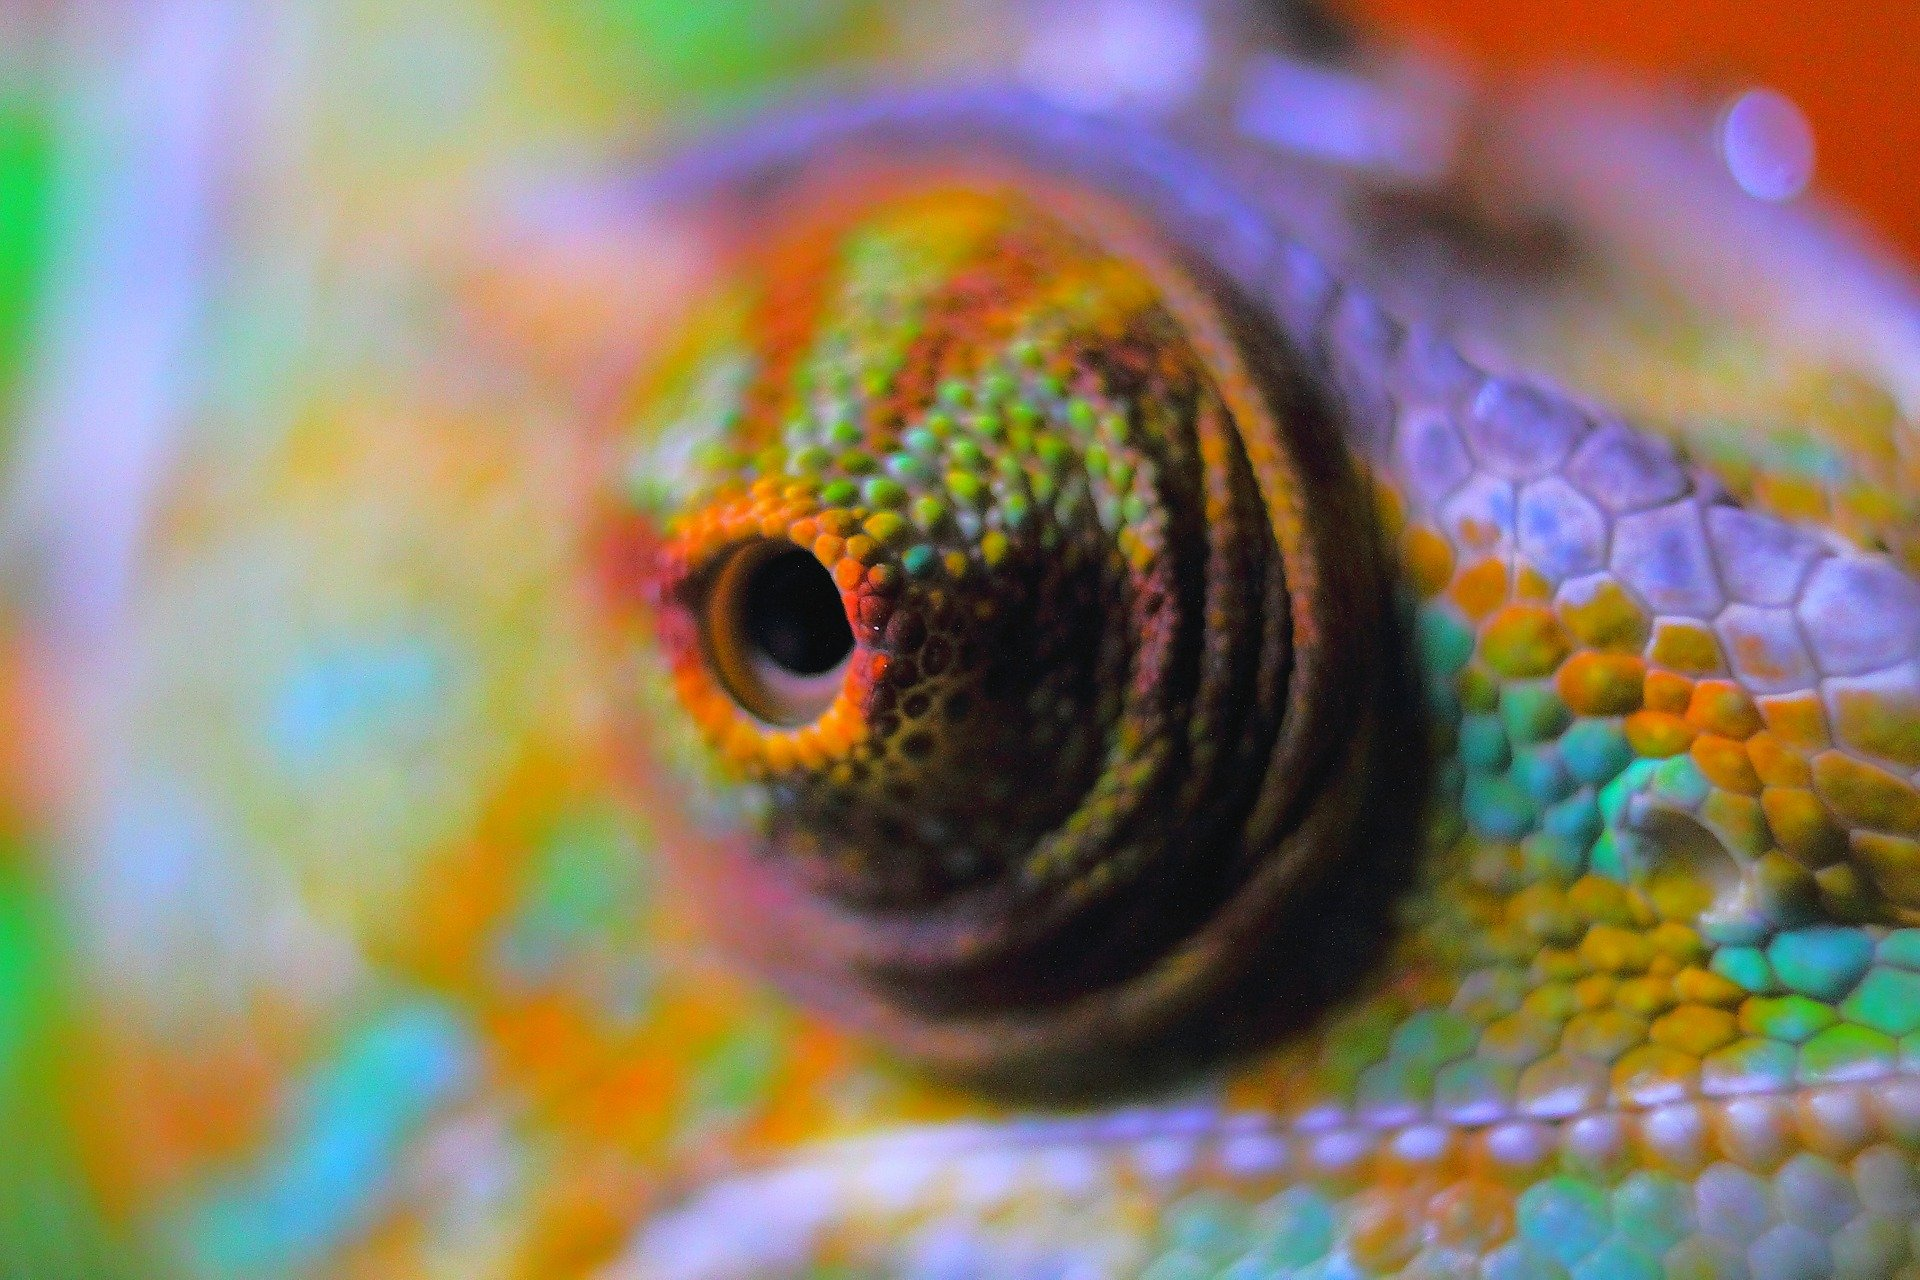
\includegraphics[width=\paperwidth]{backgrounds/img1.jpg}
}
\begin{frame}
    \frametitle{This have an bg image}
    Hello from Latex!
\end{frame}
}

% ---------------------------------------------------------------------

\begin{frame}
    \frametitle{This does not =D}
    Hello from Latex!
\end{frame}

% ---------------------------------------------------------------------

\begin{frame}
    \frametitle{A regular image}
    \centering
    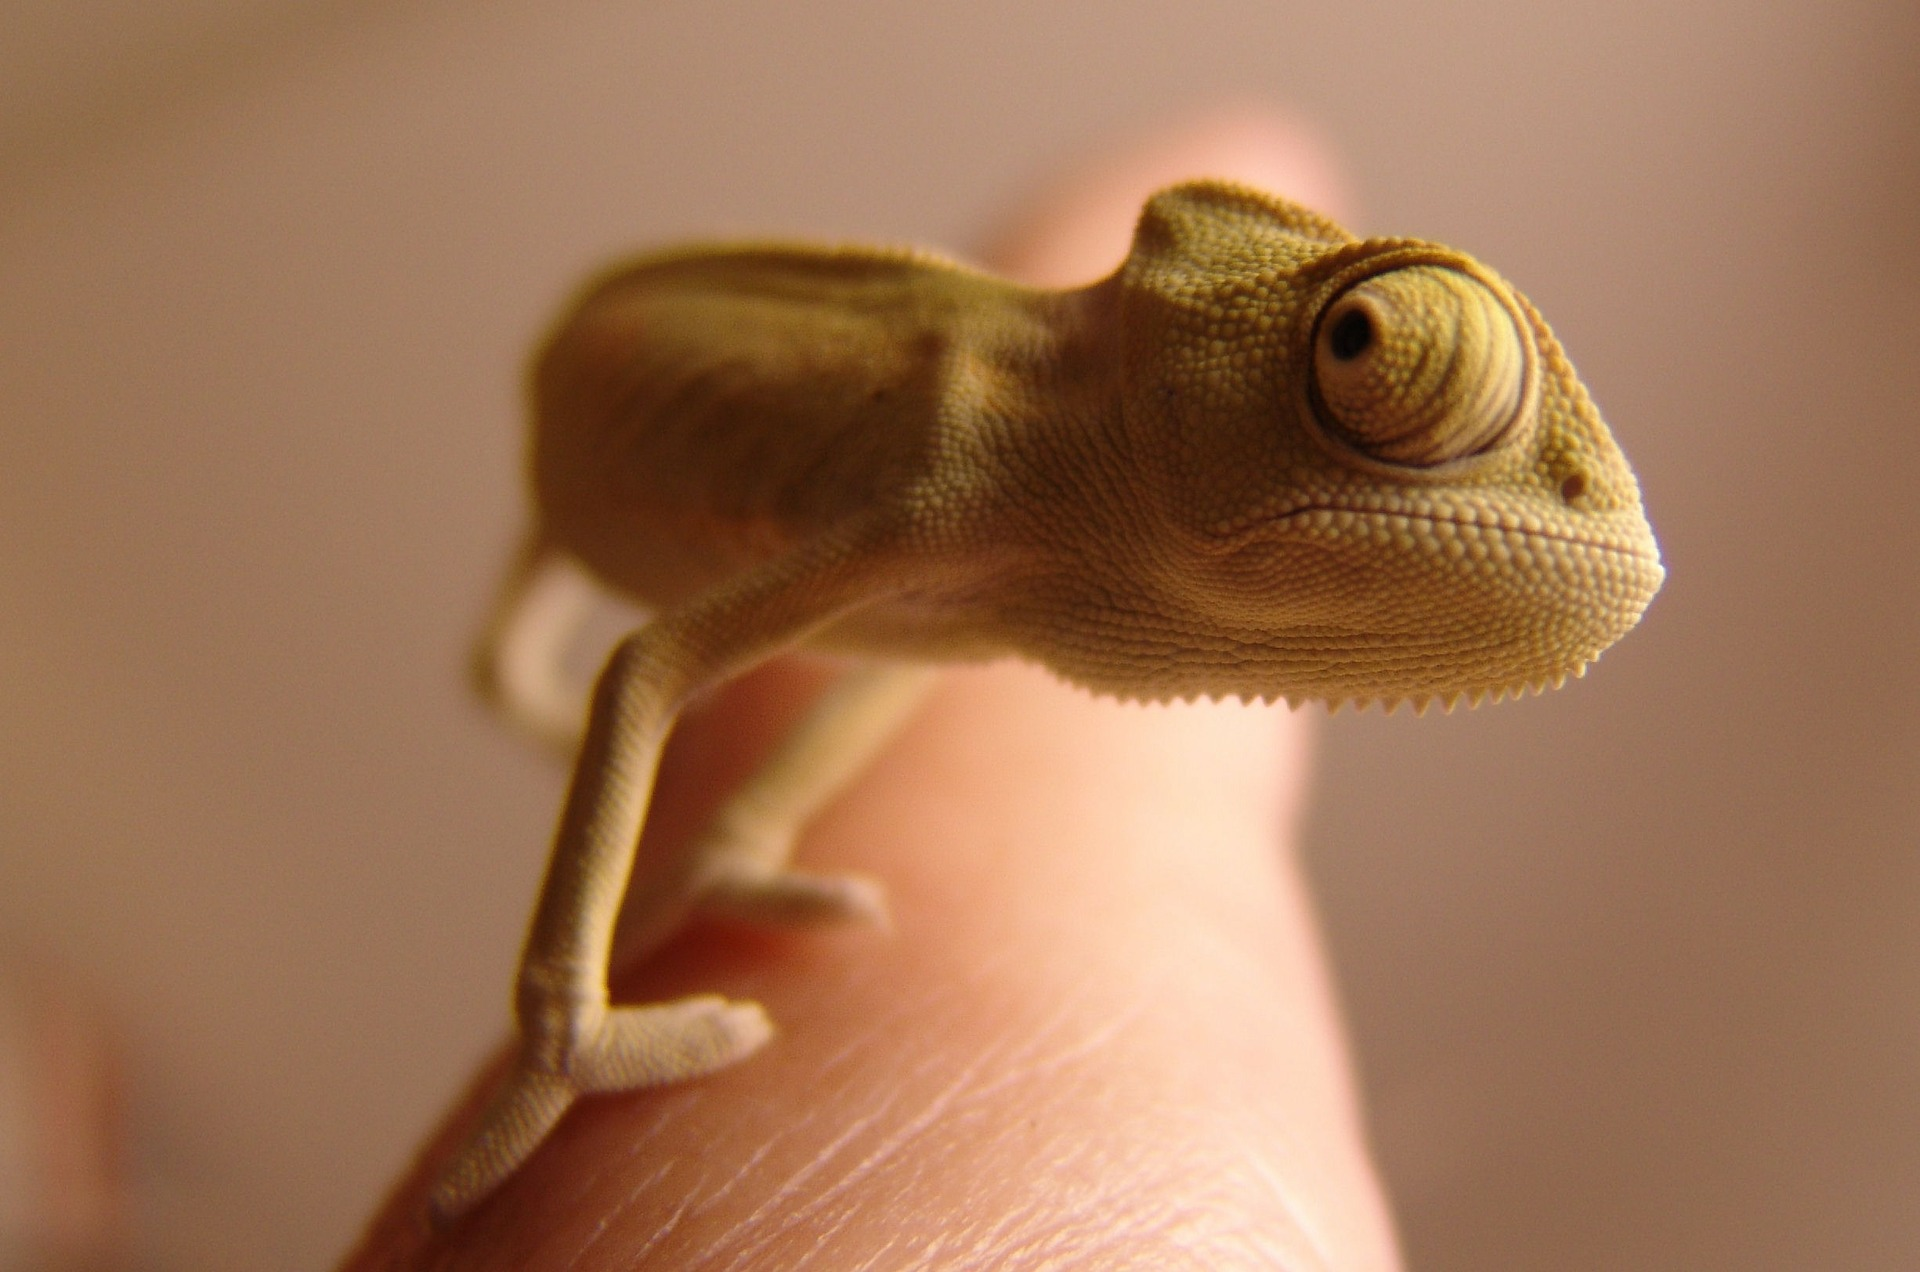
\includegraphics[width=\textwidth,height=0.6\textheight,keepaspectratio]{backgrounds/img2.jpg}
\end{frame}

% ---------------------------------------------------------------------

\begin{frame}
    \frametitle{Images in Two-column slide}
    \begin{columns}[t]
        \column{0.5\textwidth}
        \centering
        \Large{A Nice Image}\newline\newline
        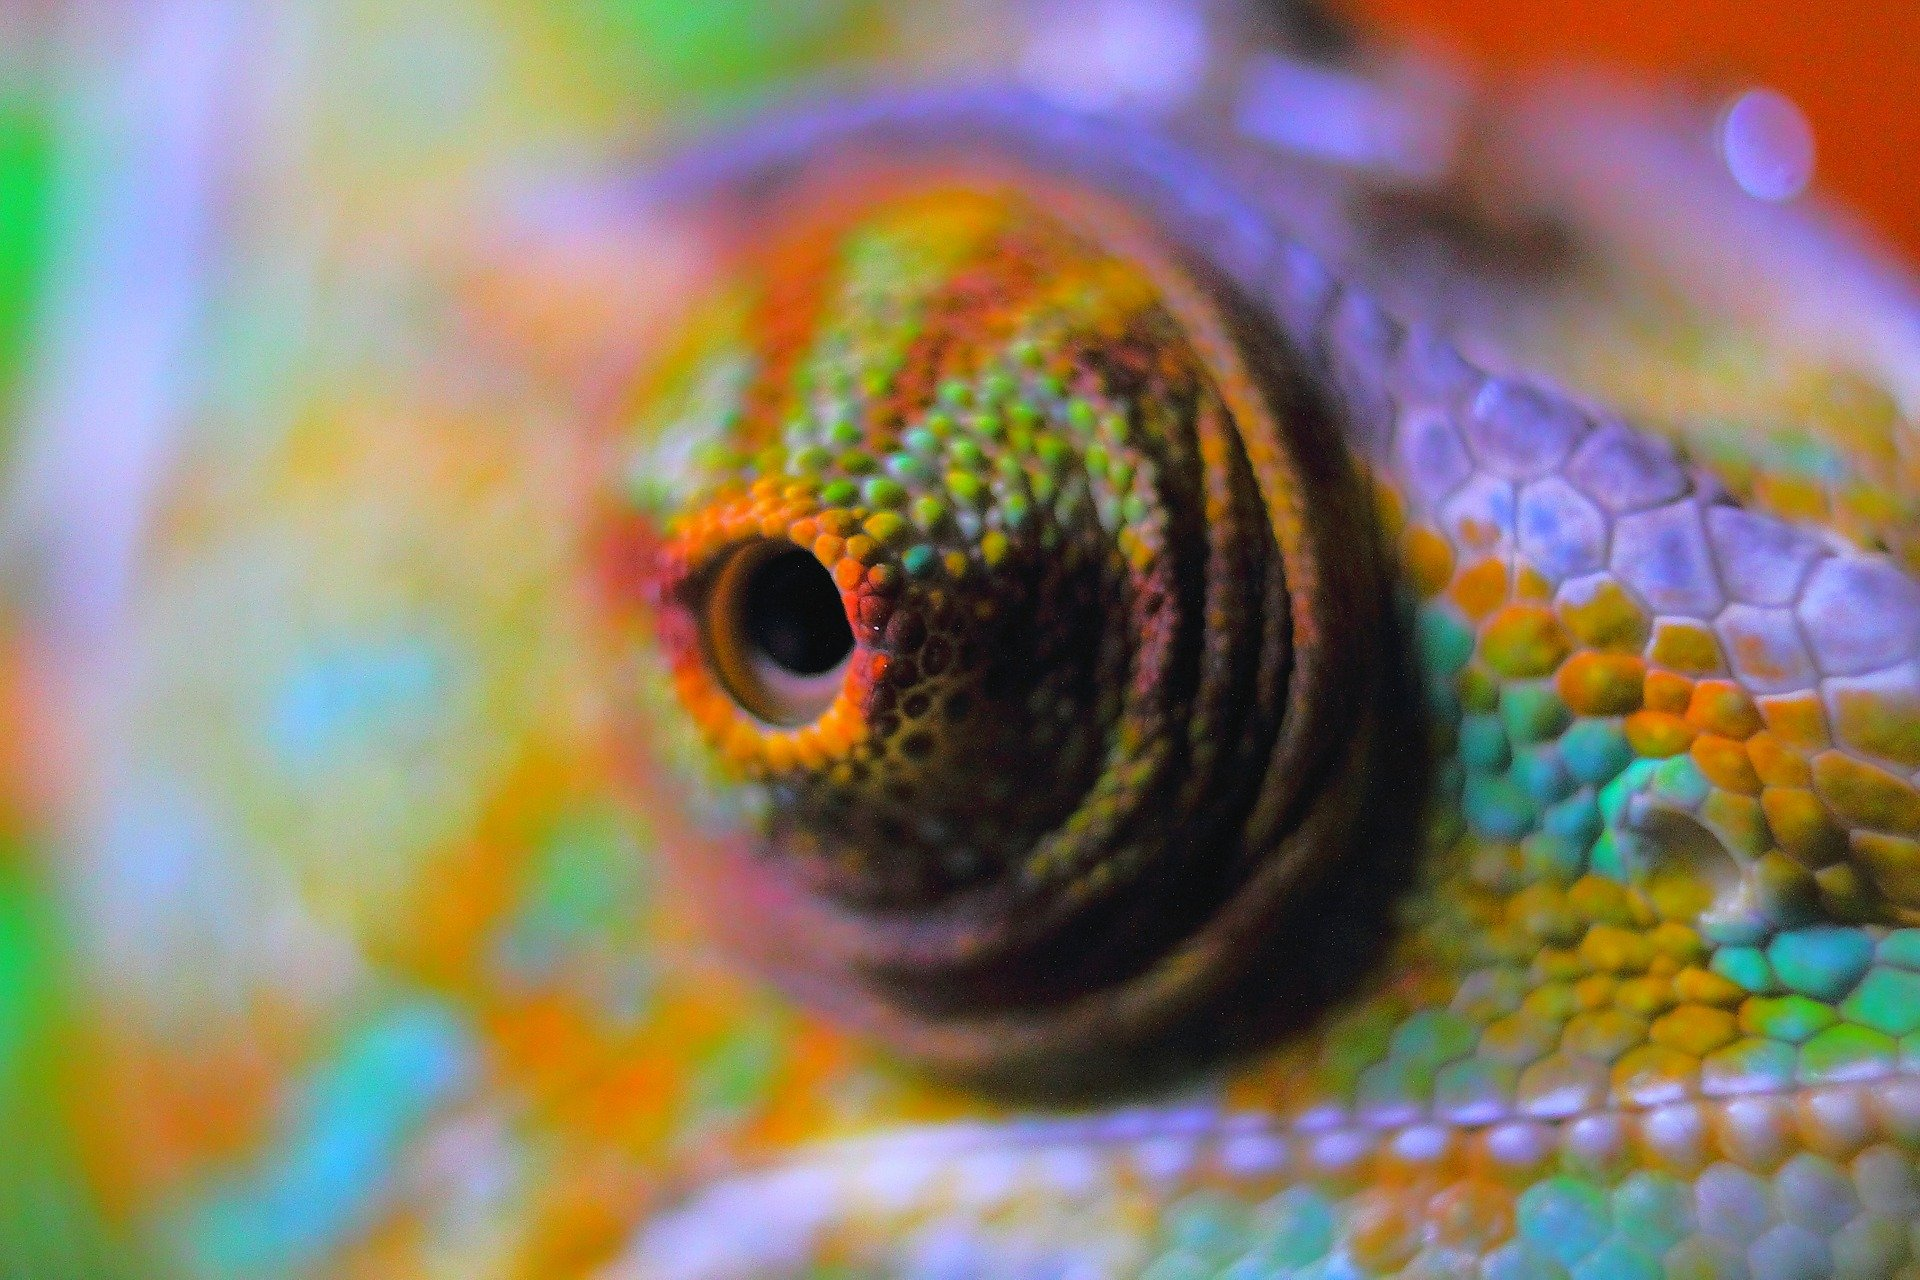
\includegraphics[width=\textwidth,height=0.5\textheight,keepaspectratio]{backgrounds/img1.jpg}
        \column{0.5\textwidth}
        \centering
        \Large{Another Image}\newline\newline
        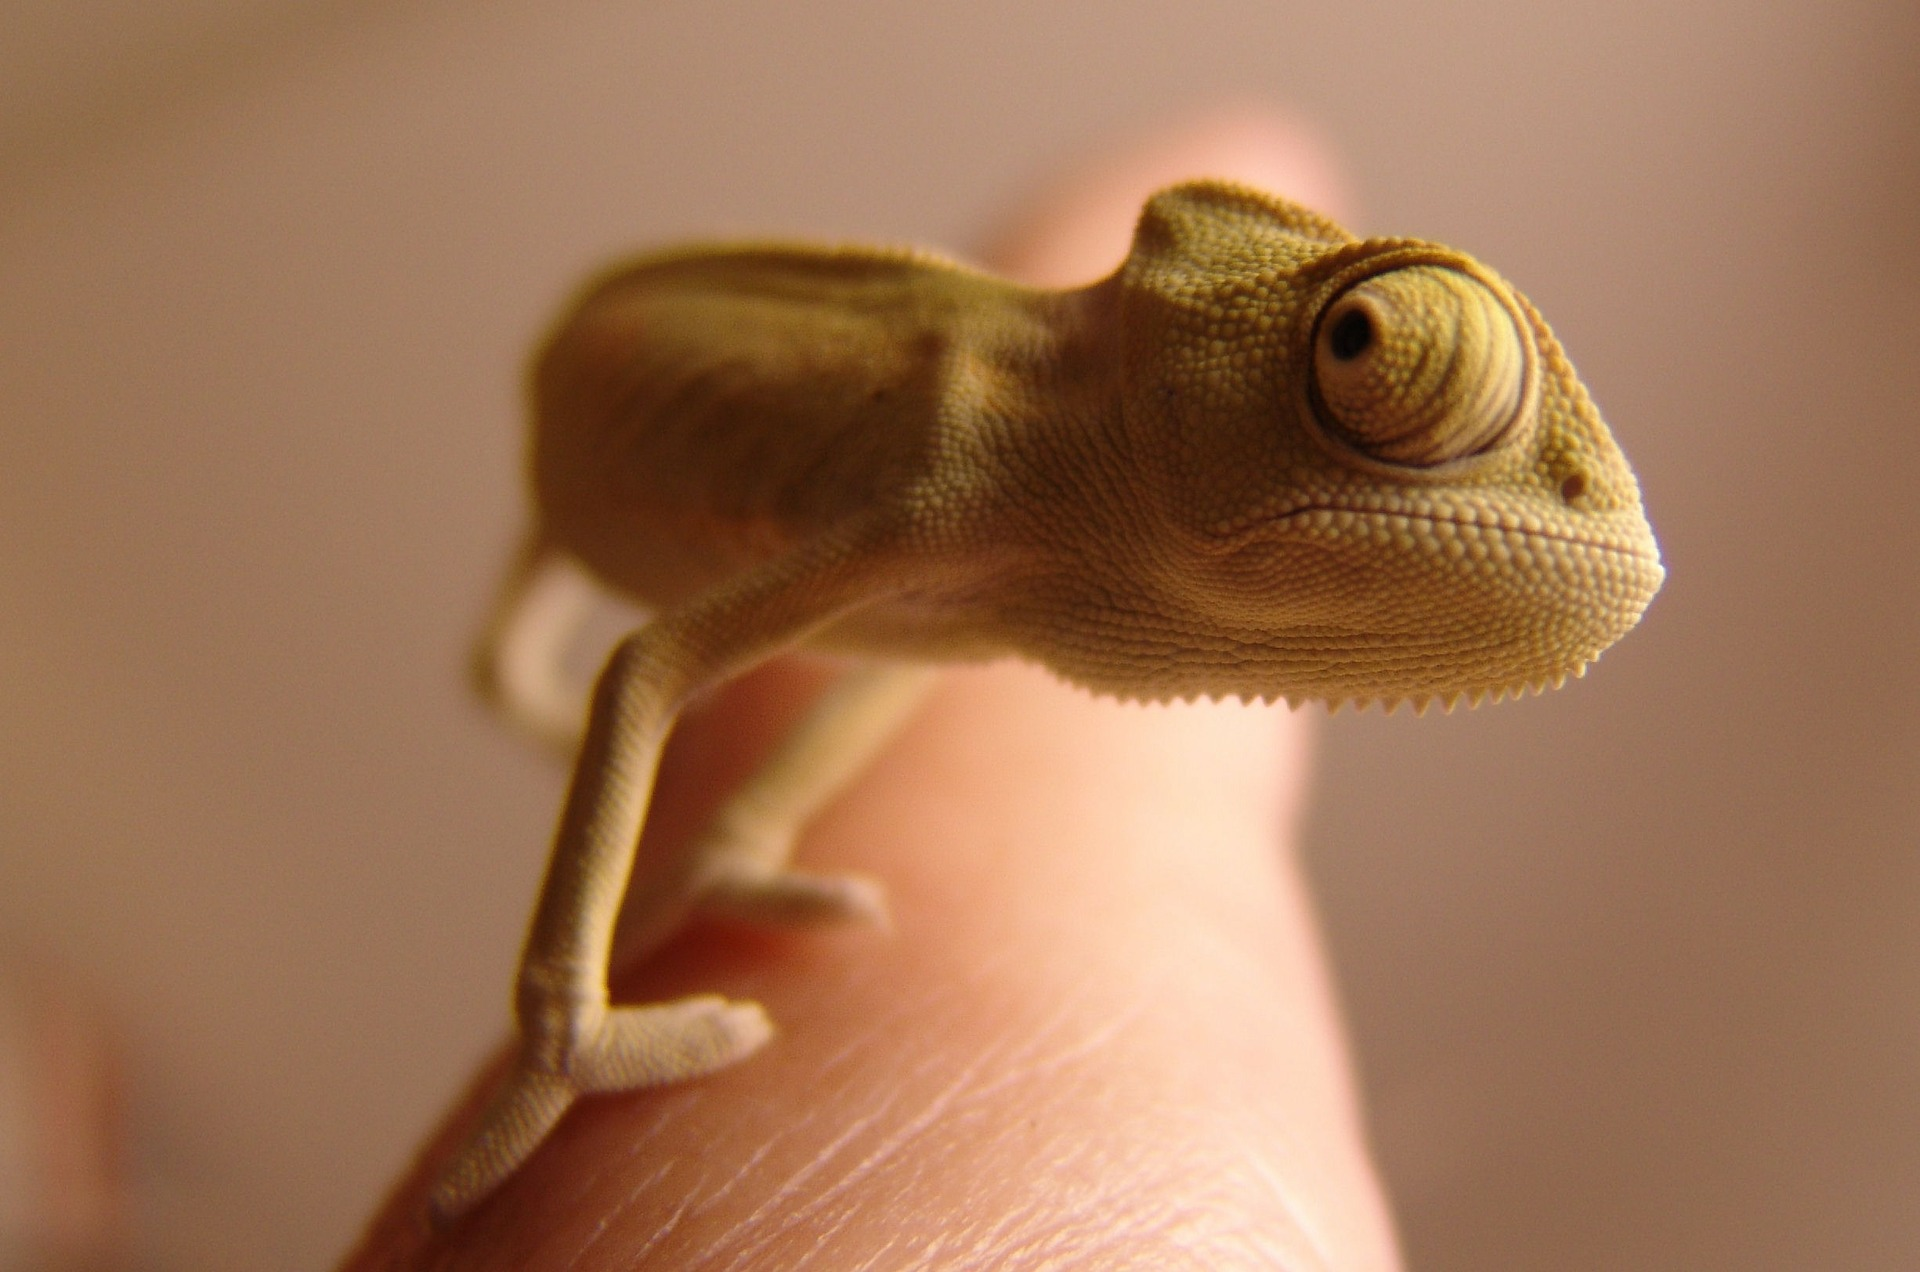
\includegraphics[width=\textwidth,height=0.5\textheight,keepaspectratio]{backgrounds/img2.jpg}
    \end{columns}
\end{frame}

% ---------------------------------------------------------------------

\begin{frame}
    \frametitle{Images + Text in Two-column slide}
    \begin{columns}[t]
        \column{0.5\textwidth}
        \centering
        \Large{A Nice Image}\newline\newline
        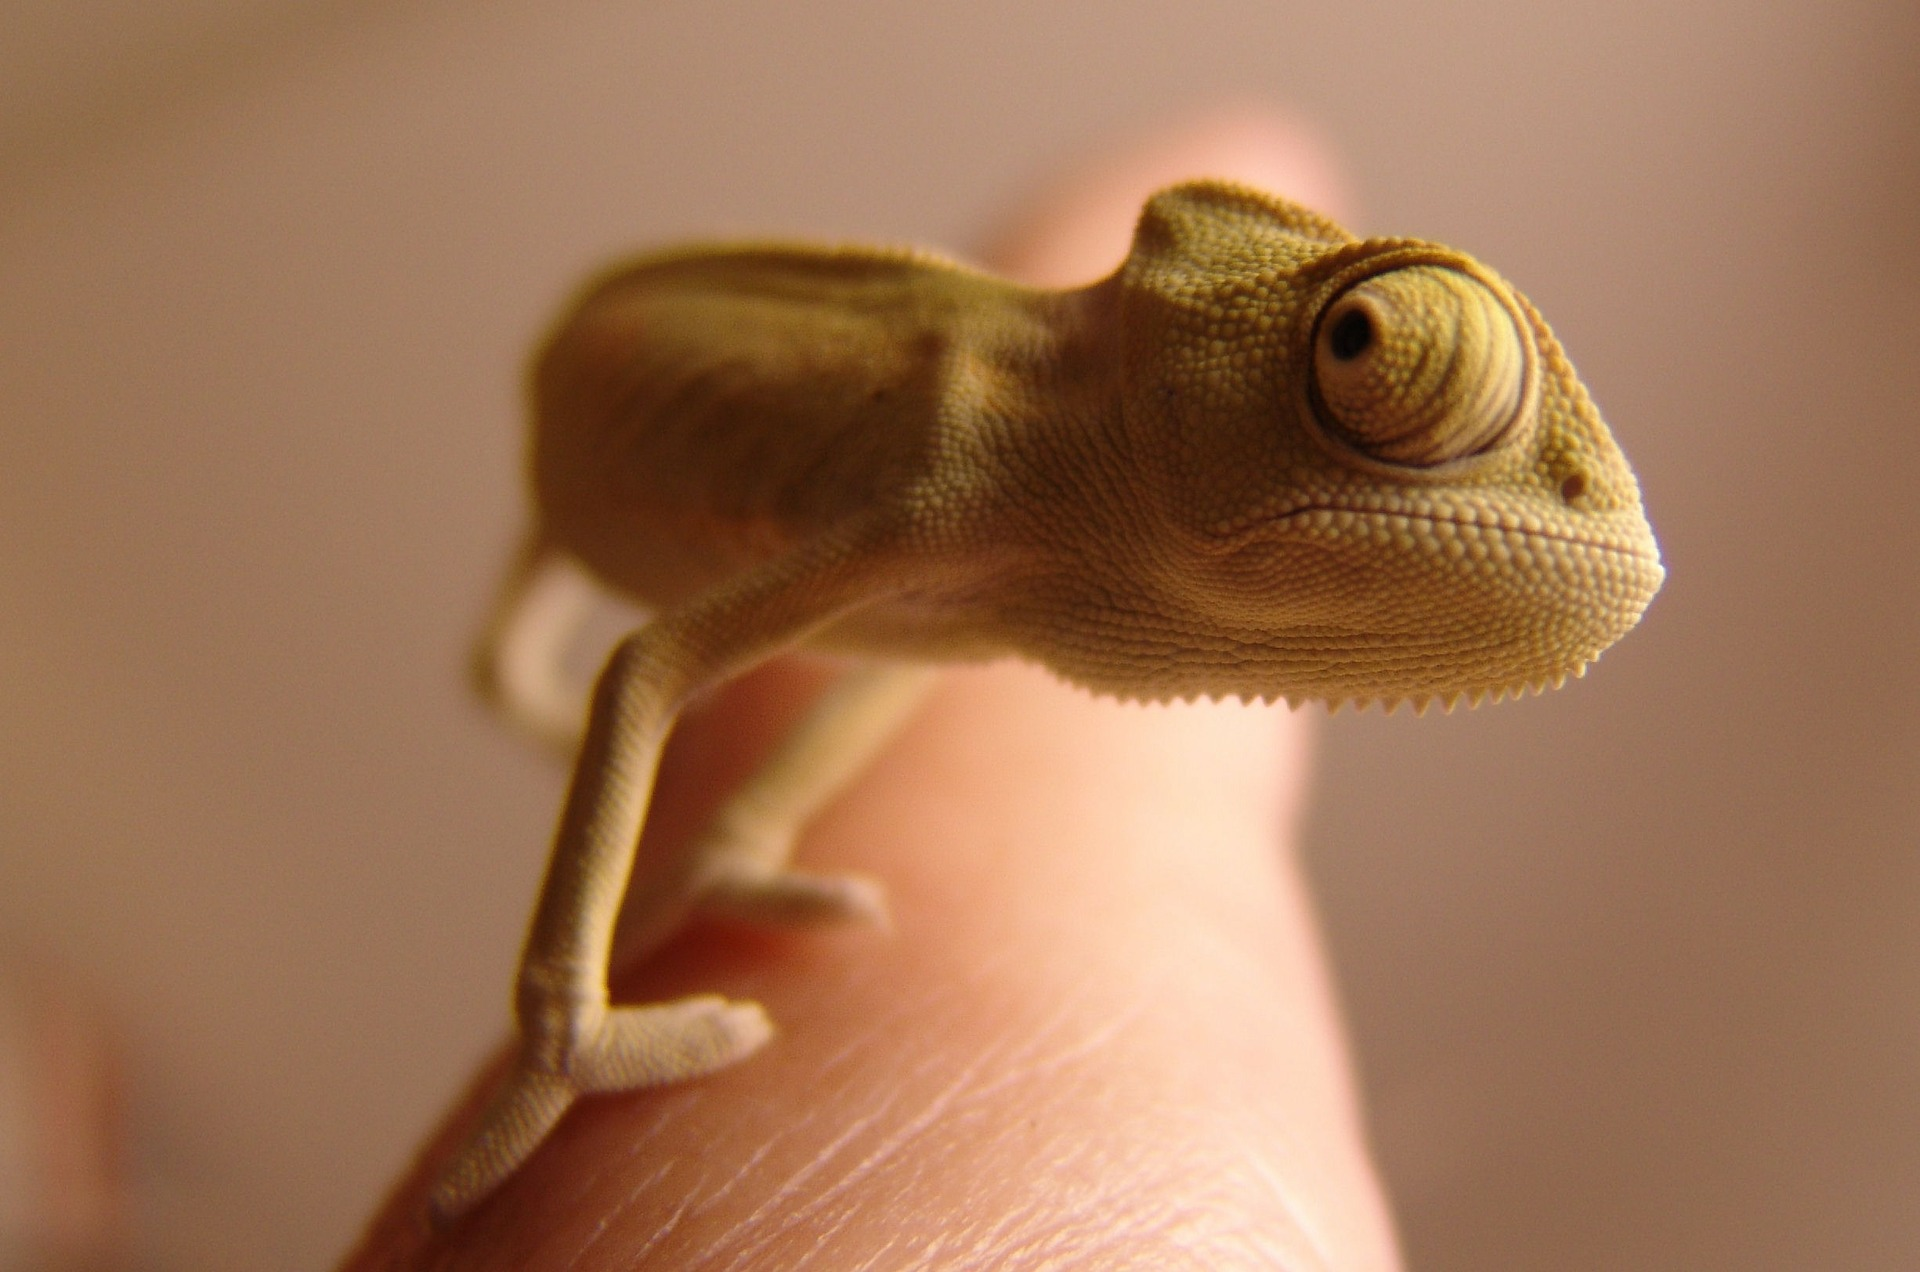
\includegraphics[width=\textwidth,height=0.5\textheight,keepaspectratio]{backgrounds/img2.jpg}
        \column{0.5\textwidth}
        \centering
        \Large{Super Text}\newline\newline
        \small{\lipsum[1][1-3]}
    \end{columns}
\end{frame}

% ---------------------------------------------------------------------

\begin{frame}
    \frametitle{Citations}

    If you want to cite some amazing book \cite{Genius1801}, or maybe
    an incredible article \cite{LaTeX2020} from the web, or even an
    amazing author \cite{SomeAuthor2022}, you can! But remember, this is
    not an article, this is a presentation.

    Acronyms like \ac{i3e} or \ac{smart} are also available.

\end{frame}

% ---------------------------------------------------------------------

\begin{frame}[t,allowframebreaks]
    \frametitle{References}
    \printbibliography
\end{frame}

% ---------------------------------------------------------------------

\begin{frame}
    \frametitle{Acronyms}
    \begin{acronym}[ICANN]
        \acro {i3e} [IEEE] {Institute of Electrical and Electronics Engineers}
\acro {smart} [SMART] {Specific, Measurable, Assignable, Realistic, Time-related}
  % <== This loads a separate list of acronyms
    \end{acronym}
\end{frame}

% ---------------------------------------------------------------------

{
\setbeamercolor{background canvas}{bg=fgcolor}
\setbeamertemplate{footline}{}
\begin{frame}
    \centering
    {\vskip 5em}
    {\color{bgcolor} \fontsize{30pt}{35pt}\selectfont Thank You!}\\
    {\vskip 3em}
    {\color{c3color} \fontsize{20pt}{25pt}\selectfont Wesley Rodrigues}\\
    {\vskip 1em}
    {\color{c3color} \fontsize{14pt}{16pt}\selectfont wesley@mymail.com}\\
    {\vskip 2em}
    
\includegraphics[width=0.35\textwidth]{logos/logo_ipt_dark_700_350.png}
\end{frame}
}

% ---------------------------------------------------------------------

\end{document}
